%   % !TEX root = ../../VIII,3_Rahmen-TeX_8-1.tex
%
%
%   Band VIII, 3 N.~??A40/Y.4
%   Signatur/Tex-Datei: LH_35_14_02_039r2
%   RK-Nr. 58234
%   Überschrift: Solidum ubique aequiresistens
%   Modul: Mechanik / Festigkeit
%   Datierung: [Ende Januar bis März/April 1683]
%   WZ: (keins)
%   SZ: (keins)
%   Bilddateien (PDF): LH_35_14_02_039r2_d1; LH_35_14_02_039r2_d2; LH_35_14_02_039r2_d3; LH_35_14_02_039r2_d4; LH_35_14_02_039r2_d5; LH_35_14_02_039r2_d6; LH_35_14_02_039r2_d7; LH_35_14_02_039r2_d8 (insgesamt: acht)
%
%
\selectlanguage{ngerman}%
\frenchspacing%
\begin{ledgroupsized}[r]{120mm}%
\footnotesize%
\pstart%
\noindent%
\textbf{Überlieferung:}%
\pend%
%
\end{ledgroupsized}%
\begin{ledgroupsized}[r]{114mm}%
\footnotesize%
\pstart%
\parindent -6mm%
\makebox[6mm][l]{\textit{L}}%
Aufzeichnung: LH~XXXV~14,~2 Bl.~39.
Ein Blatt 2\textsuperscript{o}.
Eine Seite auf Bl.~39~r\textsuperscript{o};
Bl.~39~v\textsuperscript{o} ist leer.
Bl.~39~r\textsuperscript{o} überliefert zudem N.~15. 
\pend%
\end{ledgroupsized}%
%
%
\selectlanguage{latin}%
\frenchspacing%
%
%
\vspace{8mm}
\pstart%
\noindent%
\normalsize%
%
%
\lbrack39~r\textsuperscript{o}\rbrack~Ut solidum aequaliter ubique resistat,%
\protect\index{Sachverzeichnis}{solidum ubique aequiresistens}
debet esse eadem ubique ratio momenti frangere tentantis ad%
\protect\index{Sachverzeichnis}{momentum frangere tentans}
%
\edtext{resistentiam.\protect\index{Sachverzeichnis}{resistentia solidi}
Resistentia est ut \edtext{quadratum \textit{EC},}{%
\lemma{quadratum \textit{EC}}\Cfootnote{%
Siehe das Diagramm \lbrack\textit{Fig.~1}\rbrack\ auf S.~\pageref{LH_35_14_02_039r2_Fig.1}.%
}}
pondus est area \lbrack\textit{FEC}\rbrack\ ducta}{%
\lemma{resistentiam.}\Bfootnote{%
\textit{(1)}~Sit \textit{FE}, \textit{x} \textit{CE}, \textit{y}.
\textit{(2)}~Resistentia est ut
\textit{(a)}~\textit{yy}
\textit{(b)}~quadratum \textit{EC},
\textit{(aa)}~pondus est $\displaystyle\!\int\!\!\overline{ydx}$ ductum
\textit{(bb)}~pondus est area
\textbar~\textit{FEG} \textit{ändert Hrsg.}~%
\textbar\ ducta%
~\textit{L}}}
%
in \textit{EG} distantiam centri gravitatis%
\protect\index{Sachverzeichnis}{centrum gravitatis}
%
\edtext{ab \textit{E},
vel quod}{%
\lemma{ab}\Bfootnote{%
\hspace{-0,5mm}\textit{E},
\textit{(1)}~quae habetur autem
\textit{(2)}~haec distantia
\textit{(3)}~vel quod%
~\textit{L}}}
%
idem est,
momentum ipsius \textit{FEC} ex \textit{EC} basi,
quod momentum est summa
%
\edtext{quadratorum ut \textit{HL}.\, \textit{FE}}{%
\lemma{quadratorum}\Bfootnote{%
\textit{(1)}~ipsius
\textit{(2)}~ut \textit{HL}.
\textit{(a)}~Sed \textit{F}
\textit{(b)}~\textit{EF}
\textit{(c)}~\textit{FE}%
~\textit{L}}}
%
ultima vocetur \textit{e},
et alia quaevis ut \textit{FM}
%
\edtext{vocetur \textit{x}, et \textit{ML}, \textit{y}.
Fiet $HL^2=\overline{e-x}^2$
et momentum\protect\index{Sachverzeichnis}{momentum frangere tentans}
erit \protect\rule[-4mm]{0mm}{10mm}ut $\displaystyle\!\int\!\!\overline{\overline{e-x}^2d\overline{y}}$}{%
\lemma{vocetur}\Bfootnote{%
\hspace{-0,5mm}\textit{x},
\textit{(1)}~fiet $\displaystyle\!\int\!\!\overline{\overline{e-x}^2}d\overline{y}$ ut
\textit{(2)}~et \textit{ML}, \lbrack...\rbrack\ ut $\displaystyle\!\int\!\!\overline{\overline{e-x}^2d\overline{y}}$%
~\textit{L}}}
%
quod debet esse ut \textit{yy}.
Ergo $\overline{e-x}^2dy$ ut \textit{ydy}
seu $\overline{e-x}^2=y.$
Est autem
%
\edtext{et $e=x.$
Sed hinc}{%
\lemma{et $e=x.$}\Bfootnote{%
\textit{(1)}~\textbar~Ergo fit \textit{streicht Hrsg.}~\textbar\
\textit{(a)}~$yy-2yx+xx=ay$
\textit{(b)}~\textit{yy}
\textit{(2)}~Sed hinc%
~\textit{L}}}
%
video non licere hic substituere differentialem\protect\index{Sachverzeichnis}{differentialis}
pro aequatione\protect\index{Sachverzeichnis}{aequatio summatrix}
%
\edtext{summatrice.
Item \protect\rule[-4mm]{0mm}{10mm}aliter:
$\displaystyle\!\int\!\!\overline{y\;\overline{e-x}\;dx}$ ut \textit{yy}.
Sed eodem res redit,}{%
\lemma{summatrice.}\Bfootnote{%
\textit{(1)}~Ergo aequaliter indagemus momentum quod etiam serviet, ad aequationes summatrices intractabiles ubi generalem ingreditur specialis removendas. Sed video nos in idem recidere
\textit{(2)}~\textbar~Item aliter: \textit{erg.}~%
\textbar\ $\displaystyle\!\int\!\!\overline{y\overline{e-x}dx}$ ut \textit{yy}
\textit{(a)}~ubi poste
\textit{(b)}~.~Sed eodem res redit,%
~\textit{L}}}
%
nam inventa demum summa\protect\index{Sachverzeichnis}{summa} pro \textit{e} substituere
%
% \edtext{\lbrack non\rbrack}{%
% \lemma{non}\Bfootnote{\textit{erg. Hrsg.}}}
%
licet \textit{y}.
% \pend%
%
% \pstart%
Sit ergo $y=a+bx+cxx+dx^3+hx^4$ etc.
Fiet
%
\pend%
% \newpage%
\vspace{0.3em}%
\pstart%
\noindent%
$yy\ \,=%
\begin{array}[t]{lllllllll}%
aa
& +\,2abx & +\,2acx^2 & +\,2adx^3 & +\,2ahx^4 & +2\,afx^5 & +\,2agx^6 & +\,2alx^7 & +\,2amx^8 \\
& & +\,bb & +\,2bc & +\,2bd & +\,2bh & +\,2bf & +\,2bg & +\,2bh \\
& & & & +\,cc & +\,2cd & +\,2ch & +\,2cf & +\,2cg \\
& & & & & & +\,d^2 & +\,2dh & +\,2df \\
& & & & & & & & +\,hh
\end{array}$%
\pend%
\vspace{-0.25em}
\pstart%
\noindent%
et\ \,$y \cdot \overline{e-x}\ \,=%
\begin{array}[t]{rrrrr}%
ea
& +\,ebx & +\,ecxx & +\,edx^3 & +\,ehx^4 \\
& -\,ax & -\,bxx & -\,cx^3 & -\,dx^4
\end{array}$%
\pend%
\newpage
%%%%%%%%% ACHTUNG GETRIXT: Folgende Cfootnote gehört zum Diagramm Fig.1
%%
   \centerline{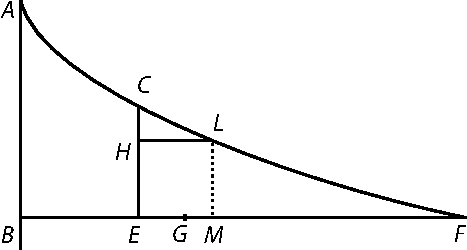
\includegraphics[width=0.5\textwidth]{gesamttex/edit_VIII,3/images/LH_35_14_02_039r2_d1.pdf}}%
  \vspace{0.5em}
  \centerline{\lbrack\textit{Fig.~1}\rbrack}%
  \label{LH_35_14_02_039r2_Fig.1}%
  \vspace{1.5em}%
%%  \newpage%

% \vspace{0.5em}%
\pstart%
\noindent
\edtext{}{%
\lemma{\hspace{1,6mm}\lbrack\textit{Fig.~1}\rbrack}%
\killnumber\Cfootnote{%
In einer ersten, nicht wiedergegebenen Fassung des Diagramms verlief die Parabel \textit{ACLF} spie\-gelverkehrt, d.h. ähnlich wie beim Diagramm \lbrack\textit{Fig.~5}\rbrack\ in N.~14\textsubscript{1}, S.~\pageref{LH_37_03_073v_Fig.5}.}}%
et
\protect\rule[-4mm]{0mm}{10mm}$\displaystyle\!\int\!\!\overline{y\;\overline{e-x}\;dx}\ \,=%
\begin{array}[t]{lllll}%
eax
& +\,\displaystyle\frac{1}{2}ebx^2 & +\,\displaystyle\frac{1}{3}ecx^3 & +\,\displaystyle\frac{1}{4}edx^4 & +\,\displaystyle\frac{1}{5}ehx^5. \\
\rule[0mm]{0mm}{6mm}%
& -\,\displaystyle\frac{1}{2}a\cdot\cdot & -\,\displaystyle\frac{1}{3}b\cdot\cdot & -\,\displaystyle\frac{1}{4}c\cdot\cdot \protect\rule[-4mm]{0mm}{10mm}& -\,\displaystyle\frac{1}{5}d\cdot\cdot
\end{array}$%
%
\pend%
\pstart%
\noindent%
Et jam pro \rule[-3mm]{0pt}{6mm}\textit{e} substituendo \textit{x},
fiet:
$\displaystyle\frac{1}{2}axx+\displaystyle\frac{1}{6}bx^3+\displaystyle\frac{1}{12}cx^4+\displaystyle\frac{1}{20}dx^5+\displaystyle\frac{1}{30}hx^6$
quae est ut \textit{yy}.
%
Ergo $a=0,$ ob \textit{aa} cui nil respondet.
Ergo et $\displaystyle\frac{1}{2}axx=0,$
et $2acx^2=0,$
et $bbxx=0.$
Ergo et $\displaystyle\frac{1}{6}bx^3=0,$
quod et esse \rule[-3mm]{0pt}{6mm}debet quia $2a\;\overline{d+bc}\;x^3=0.$
Fit ergo $ccx^4$
\edlabel{LH_35_14_02_039r2_f039r1}ut
$\displaystyle\frac{1}{12}cx^4.$%
\edtext{}{%
{\xxref{LH_35_14_02_039r2_f039r1}{LH_35_14_02_039r2_f039r2}}%
{\lemma{ut $\displaystyle\frac{1}{12}cx^4.$}\Bfootnote{%
\textit{(1)}~Quod verum est. Caeterum hinc videntur infinitae aliae curvae haberi posse idem praest
\textit{(2)}~Et locus ad parabolam.%
~\textit{L}}}}
%
Et locus ad \edlabel{LH_35_14_02_039r2_f039r2}parabolam.\protect\index{Sachverzeichnis}{parabola}
\pend%
%
\pstart%
Si caeteras omnes literas\protect\index{Sachverzeichnis}{litera} ponamus $=0,$
videamus tamen an et alio modo solvi problema possit,
faciendo verbi gratia omnes literas $=0$ praeter \textit{c} et \textit{d}.
Et fiet $ccx^4+2cdx^5+ddx^6$
ut \rule[-3mm]{0pt}{6mm}
$\displaystyle\frac{1}{12}cx^4+\displaystyle\frac{1}{20}dx^5+\displaystyle\frac{1}{30}hx^6,$
seu multiplicando posteriorem
formulam\protect\index{Sachverzeichnis}{formula}
per $12c$
fiet $ccx^4+2cdx^5+ddx^6$
ut \rule[-3mm]{0pt}{6mm}$ccx^4+\displaystyle\frac{12cd}{20}%
\edtext{\lbrack x^5\rbrack}{\lemma{$x^5$}\Bfootnote{\textit{erg. Hrsg.}}}%
+\displaystyle\frac{12ch}{30}x^6$ etc.
quod fieri non potest.
Et vero resolvamus aeq. generaliter,
fiet \rule[-3mm]{0pt}{6mm}$ccx^4 + \displaystyle\frac{12cd}{20}x^5 + \displaystyle\frac{12}{30}chx^6 + \displaystyle\frac{12cf}{42}x^7 + \displaystyle\frac{12cg}{56}x^8$
etc.
\makebox[1.0\textwidth][s]{$=%
\begin{array}[t]{llll}%
c^2x^4 + 2cdx^5 & +\, 2chx^6 & +\, 2cfx^7 & +\, 2cgx^8 \\
& +\, dd & +\, 2dh & +\, 2df \\
& & & +\, hh
\end{array}$
etc.
et fit $d=0.$
Ergo et $h=0.$
Ergo et}
\pend
\newpage
\pstart
\noindent $g=0.$
Et ita credo porro in infinitum.\protect\index{Sachverzeichnis}{infinitum}
Nec alius casus\protect\index{Sachverzeichnis}{casus} datur.
Sit ergo
%
\edtext{\textit{FE}, \textit{x}, et \textit{EC}, \textit{y}.}{%
\lemma{\textit{FE}, \textit{x}, et \textit{EC}, \textit{y}}\Cfootnote{%
Siehe \lbrack\textit{Fig~1}\rbrack\ auf S.~\pageref{LH_35_14_02_039r2_Fig.1}.}}
%
Et $y = xx : r.$
Videamus an res
%
\edtext{succedat. \textit{yy} est}{%
\lemma{succedat.}\Bfootnote{%
\textit{(1)}~Constat \textit{yy} esse
\textit{(2)}~\textit{yy} est%
~\textit{L}}}
%
ut $x^4,$
area parabolae\protect\index{Sachverzeichnis}{parabola} est
\rule[-0mm]{0pt}{6mm}%
$\displaystyle\frac{1}{3}yx$
seu ut $x^3.$
At \textit{EG} est ut \textit{x}
seu certa pars ipsius \textit{x}.
%
Nam%
\edlabel{LH_35_14_02_039r_integralfaktor-1}
%
\edtext{$\displaystyle\!\!\int\!\!\overline{xydx}$ momentum%
\protect\index{Sachverzeichnis}{momentum ex vertice}
ex vertice\protect\index{Sachverzeichnis}{vertex}%
\edlabel{LH_35_14_02_039r_integralfaktor-2}
est
ut $\displaystyle\!\!\int\!\!\overline{x^3dx}$ seu ut $\displaystyle\frac{1}{4}x^4,$
quod divisum}{%
\lemma{$\displaystyle\!\int\!\!\overline{xydx}$}\Bfootnote{%
\textit{(1)}~est ut
\textit{(2)}~momentum ex
\textit{(a)}~axe
\textit{(b)}~vertice est ut $\displaystyle\!\int\!\!\overline{x^3dx}$
\textit{(aa)}~seu ut $x^4,$ quod div
\textit{(bb)}~seu ut $\displaystyle\frac{1}{4}x^4,$
\textit{(aaa)}~quae
\textit{(bbb)}~quod divisum%
~\textit{L}}}
%
per aream
\rule[-3mm]{0pt}{6mm}%
$\displaystyle\frac{1}{3}x^3$
dat $\displaystyle\frac{3}{4}x=FG,$
ergo $EG=\displaystyle\frac{1}{4}x.$
%
Ergo
%
\edtext{Area ut $x^3,$ ducta in}{%
\lemma{Area}\Bfootnote{%
\textit{(1)}~ducta in
\textit{(2)}~ut $x^3,$ ducta in%
~\textit{L}}}
%
\textit{EG}, quae est ut \textit{x},
erit ut $x^4$ seu ut \textit{yy}.
\pend%
%
\pstart%
%
\edtext{Galilaeus%
\protect\index{Namensregister}{\textso{Galilei} (Galilaeus, Galileus), Galileo 1564\textendash1642}
alio sensu corpus aequaliter resistens accipit,%
\protect\index{Sachverzeichnis}{corpus aequaliter resistens}
ut
%
\edtext{scilicet trabs\protect\index{Sachverzeichnis}{trabs ubique aequiresistens}
corpori% \lbrack corpore\rbrack\
}{%
\lemma{scilicet}\Bfootnote{%
\textit{(1)}~corpori
\textit{(2)}~trabs corpori%
% \textbar~corpori \textit{ändert Hrsg.}~%
% \textbar\ in extremitate appenso%
~\textit{L}}}
%
in extremitate appenso\protect\index{Sachverzeichnis}{corpus appensum}
ubique aequaliter resistat,
abstrahendo ab ipsius pondere proprio.%
\protect\index{Sachverzeichnis}{pondus proprium}}{%
\lemma{Galilaeus \lbrack...\rbrack\ proprio}\Cfootnote{%
Zur Gestalt des gleichmäßig widerstandsfähigen Balkens siehe G.\,\textsc{Galilei}, \textit{Discorsi}, Leiden 1638, S.~137–141\cite{00050} (\textit{GO} VIII, S.~177–181).\cite{00048}
Für die Annahme, dass vom Eigengewicht des Balkens zu abstrahieren sei,
siehe ebd., S.~115\cite{00050} (\textit{GO} VIII, S.~157.13\textendash20).\cite{00048}
Leibniz hatte sich mit Galileis Fragestellung bereits in Paris auseinandergesetzt;
vgl. \textit{LSB} VIII,~2 N.~22.\cite{01252}}}
%
Et hoc problema\protect\index{Sachverzeichnis}{problema} longe est facilius.
Non est enim opus dimensione\protect\index{Sachverzeichnis}{dimensio figurae}
et centro gr. ipsius figurae.\protect\index{Sachverzeichnis}{centrum gravitatis figurae}
%
\edtext{\lbrack Debent\rbrack}{%
\lemma{Debet}\Bfootnote{%
\textit{L~ändert Hrsg.}}}
%
scilicet
%
\edtext{esse \textit{AC} ipsis $BC^2$ proportionales
seu \textit{x} ut $y^2.$}{%
\lemma{esse}\Bfootnote{%
\textit{(1)}~\textit{AB} ad $BC^2$ in eadem ratione seu \textlangle ut\textrangle\
\textit{(2)}~\textit{AC} ipsis \lbrack...\rbrack\ ut $y^2.$% $BC^2$ proportionales seu \textit{x}
~\textit{L}}}
%
Ergo figura\protect\index{Sachverzeichnis}{figura}
est parabola\protect\index{Sachverzeichnis}{parabola}
quod est facillimum.%
\pend%
%%
%%
%%  \newpage% 
% \vspace{2.0em}%	% Diagramm Fig~2
%  \centerline{\hspace*{-55mm}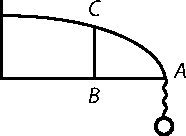
\includegraphics[width=0.23\textwidth]{gesamttex/edit_VIII,3/images/LH_35_14_02_039r2_d2.pdf}}%
%  \vspace{-0.5em}
%  \centerline{\hspace*{-60mm}\lbrack\textit{Fig.~2}\rbrack}%
%  \label{LH_35_14_02_039r2_Fig.2}%
%%  \vspace{1.5em}%
%%  \newpage%
%%
%%  \newpage% 
% \vspace{-7.5em}%	% Diagramm Fig.~3
%  \centerline{\hspace*{55mm}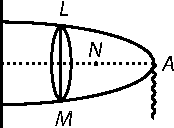
\includegraphics[width=0.16\textwidth]{gesamttex/edit_VIII,3/images/LH_35_14_02_039r2_d3.pdf}}%
%  \vspace*{0.5em}
%  \centerline{\hspace*{55mm}\lbrack\textit{Fig.~3, gestr.}\rbrack}%
%  \label{LH_35_14_02_039r2_Fig.3}%
%  \vspace{2.5em}%
%%  \newpage%
%%
%
\vspace{1em}
\pstart%
\noindent%
\lbrack\textit{Nachfolgend kleingedruckter Text in L gestrichen:}\rbrack\
\pend%
\vspace{0.5em}
\pstart%
\footnotesize%
Ponamus\edlabel{LH_35_14_02_039r2_Rotationskoerper_kdfgh-1}
quaeri corpus rotatione
genitum\protect\index{Sachverzeichnis}{corpus rotatione genitum}
conforme\protect\index{Sachverzeichnis}{corpus conforme}
quod ubique aequaliter resistat%
\protect\index{Sachverzeichnis}{corpus ubique aequiresistens}%
\lbrack;\rbrack\
resistentia\protect\index{Sachverzeichnis}{resistentia corporis}
cujusque circuli est ut circulus\lbrack,\rbrack\
%
\edtext{si sc. \textit{LM} ductus}{%
\lemma{si}\Bfootnote{%
\hspace{-0,5mm}sc.
\textit{(1)}~ductus
\textit{(2)}~\textit{LM} ductus%
~\textit{L}}}
%
in \textit{LN} distantiam centri gravitatis a basi,%
\protect\index{Sachverzeichnis}{distantia centri gravitatis}
id est ut cubi \edlabel{LH_35_14_02_039r2_f039r3}diametrorum.%
\edlabel{LH_35_14_02_039r2_Rotationskoerper_kdfgh-2}%
\edtext{}{%
{\xxref{LH_35_14_02_039r2_f039r3}{LH_35_14_02_039r2_f039r4}}%
{\lemma{diametrorum.}\Bfootnote{%
\textit{(1)}~Ergo debet \textit{AN}
\textit{(2)}~Sed quid si%
~\textit{L}}}}
\pend
%%%%%%%%%%%%%%%%%%%%%%%%Abbildungen 2 und 3%%%%%%%%%%%%%%%%%%%%%%%%%%%%%%%%%%%%%%
\vspace{-0.2em} 
\pstart\setline{1}
\begin{minipage}[t]{0.5\textwidth}
\hspace{10mm}
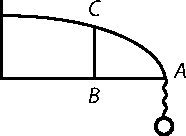
\includegraphics[width=0.47\textwidth]{gesamttex/edit_VIII,3/images/LH_35_14_02_039r2_d2.pdf}
\end{minipage}
\hspace{15mm}
\begin{minipage}[t]{0.5\textwidth}
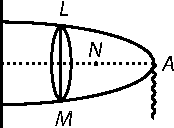
\includegraphics[width=0.37\textwidth]{gesamttex/edit_VIII,3/images/LH_35_14_02_039r2_d3.pdf}
\end{minipage}
\\
\\
\hspace*{26mm} [\textit{Fig.~2}] \label{LH_35_14_02_039r2_Fig.2}\hspace*{52mm} [\textit{Fig.~3, gestr.}]\label{LH_35_14_02_039r2_Fig.3}%
\pend
\newpage%
%
\pstart%
Sed quid si\edlabel{LH_35_14_02_039r2_f039r4}
\lbrack\textit{Text bricht ab.}\rbrack%
\pend%
% \newpage%
%
% % % % % %     A C T H U N G   G E T R I X T     % % % % % %
%
%    Die folgende Cfootnote hängt mit den Abbildungen Fig.4 bis Fig.8 zusammen !!!!
%
% % % % % %     A C T H U N G   G E T R I X T     % % % % % %
%
\pstart%
\edtext{}{%
\lemma{\hspace{1,6mm}\lbrack\textit{Fig.~4}\rbrack\ und \lbrack\textit{Fig.~5}\rbrack}\killnumber\Cfootnote{%
Wahrscheinlich Entwürfe zu den Diagrammen
\lbrack\textit{Fig.~7}\rbrack\ und
\lbrack\textit{Fig.~10}\rbrack\ bis \lbrack\textit{Fig.~12}\rbrack\
in N.~14\textsubscript{2},
S.~\pageref{LH_37_03_070r_d07}f. % ,
% \pageref{LH_37_03_070r_Fig.10},
u.~\pageref{LH_37_03_070v_Fig.11}f. % und
% \pageref{LH_37_03_070v_Fig.12c}.
}}%
\edtext{}{%
\lemma{\hspace{1,6mm}\lbrack\textit{Fig.~6}\rbrack\ und \lbrack\textit{Fig.~7}\rbrack}\killnumber\Cfootnote{%
Wahrscheinlich Entwürfe zum Diagramm
\lbrack\textit{Fig.~3}\rbrack\
in N.~14\textsubscript{1},
S.~\pageref{LH_37_03_073r_Fig.3}.}}%
\pend%
%Abbildungen 4 bis 6 %%%%%%%%%%%%%%%%%%%%%%%%%%%%%%%%%%%%%%%%%%%%%%%%%%%%%%%%%%%%%%%%%%
\pstart\noindent
\hspace{-7mm}\begin{minipage}[t][6.2cm][c]{0.25\textwidth}
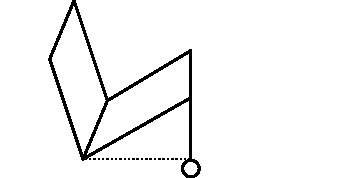
\includegraphics[width=1.7\textwidth]{gesamttex/edit_VIII,3/images/LH_35_14_02_039r2_d4.pdf}
\end{minipage}
\hspace{17mm}
\begin{minipage}[t][6.2cm][c]{0.25\textwidth}
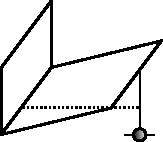
\includegraphics[width=0.8\textwidth]{gesamttex/edit_VIII,3/images/LH_35_14_02_039r2_d5.pdf}
\end{minipage}
\hspace{8mm}
\begin{minipage}[t][6.2cm][c]{0.5\textwidth}
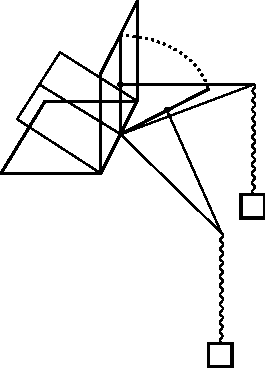
\includegraphics[width=0.66\textwidth]{gesamttex/edit_VIII,3/images/LH_35_14_02_039r2_d6.pdf}
\end{minipage}
\\
\\
\hspace*{3mm} [\textit{Fig. 4}]\label{LH_35_14_02_039r2_Fig.4}\hspace*{34mm} [\textit{Fig. 5}] \label{LH_35_14_02_039r2_Fig.5}\hspace*{36mm} [\textit{Fig. 6}]\label{LH_35_14_02_039r2_Fig.6}
\vspace{1em}
\pend
%%%%%%%%%%%%%%%%%%%%%%%%%%%%%%%%%%%%%%%%%%%%%%%%%%%%%%%%%%%%%%%%%%%%%%%%%%%
%%  \newpage% 
% \vspace*{1.5em}%	% Diagramm Fig.~4
%  \centerline{\hspace*{-45mm}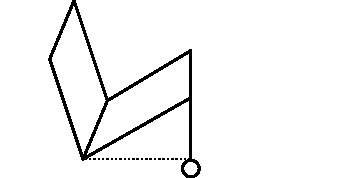
\includegraphics[width=0.42\textwidth]{gesamttex/edit_VIII,3/images/LH_35_14_02_039r2_d4.pdf}}%
%  \vspace*{0.5em}
%  \centerline{\hspace*{-65mm}\lbrack\textit{Fig.~4}\rbrack}%
%  \label{LH_35_14_02_039r2_Fig.4}%
%%  \vspace{2em}%
%%  \newpage%
%%
%%  \newpage% 
% \vspace{-9.5em}%	% Diagramm Fig.~5
%  \centerline{\hspace*{45mm}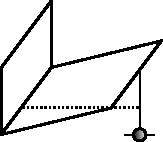
\includegraphics[width=0.20\textwidth]{gesamttex/edit_VIII,3/images/LH_35_14_02_039r2_d5.pdf}}% 
%  \vspace*{1.0em}
%  \centerline{\hspace*{40mm}\lbrack\textit{Fig.~5}\rbrack}% 
%  \label{LH_35_14_02_039r2_Fig.5}%
%%  \vspace{2em}%
%%  \newpage%
%%
%%  \newpage% 
% \vspace{1.5em}%	% Diagramm Fig.~6
%  \centerline{\hspace*{-85mm}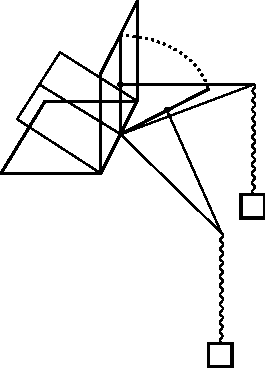
\includegraphics[width=0.34\textwidth]{gesamttex/edit_VIII,3/images/LH_35_14_02_039r2_d6.pdf}}%
%  \vspace*{-8.0em}
%  \centerline{\hspace*{-90mm}\lbrack\textit{Fig.~6}\rbrack}%
%  \label{LH_35_14_02_039r2_Fig.6}%
%%  \vspace{2em}%
%%  \newpage%
%
%  \newpage% 
%%%%%%%%%%%%%%%%%%%%%%%%%%%Abbildungen 7 und 8 %%%%%%%%%%%%%%%%%%%%%%%%%%%%%%%%%%%
\vspace{1.5em} 
\pstart \setline{1}
\hspace{12mm}\begin{minipage}[t]{0.5\textwidth}
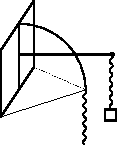
\includegraphics[width=0.46\textwidth]{gesamttex/edit_VIII,3/images/LH_35_14_02_039r2_d8.pdf}
\end{minipage}
\hspace{1mm}
\begin{minipage}[t]{0.5\textwidth}
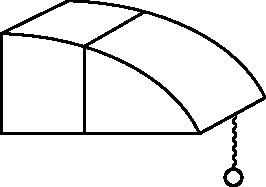
\includegraphics[width=0.47\textwidth]{gesamttex/edit_VIII,3/images/LH_35_14_02_039r2_d7.pdf}
\end{minipage}
\\
\\
\hspace*{26mm} [\textit{Fig.~7}]\label{LH_35_14_02_039r2_Fig.7}\hspace*{58mm} [\textit{Fig.~8}]\label{LH_35_14_02_039r2_Fig.8}
\pend
%%%%%%%%%%%%%%%%%%%%%%%%%%%%%%%%%%%%%%%%%%%%%%%%%%%%%%%%%%%%%%%%%%%%%%%%%%
%\vspace{1em}
%
% \vspace{-10.0em}%	% Diagramm Fig.~7
%  \centerline{\hspace*{100mm}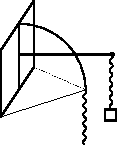
\includegraphics[width=0.16\textwidth]{gesamttex/edit_VIII,3/images/LH_35_14_02_039r2_d8.pdf}}%
%  \vspace*{0.5em}
%  \centerline{\hspace*{95mm}\lbrack\textit{Fig.~7}\rbrack}%
%  \label{LH_35_14_02_039r2_Fig.7}%
%%  \vspace{2em}%
%%  \newpage%
%%
%%  \newpage% 
% \vspace{2.0em}%	% Diagramm Fig.~8
%  \centerline{\hspace*{40mm}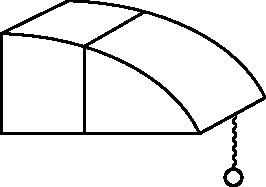
\includegraphics[width=0.32\textwidth]{gesamttex/edit_VIII,3/images/LH_35_14_02_039r2_d7.pdf}}%
%  \vspace*{0.5em}
%  \centerline{\hspace*{40mm}\lbrack\textit{Fig.~8}\rbrack}%
%  \label{LH_35_14_02_039r2_Fig.8}%
%%  \vspace{2em}%
%%  \newpage%
%
%
% % % %  Ende dest Textes auf Bl. 39r
%
%
% \newpage%
\count\Bfootins=1200
\count\Afootins=1200
\count\Cfootins=1200
%
%